% Preamble
% ---
\documentclass{article}

% Packages
% ---
\usepackage{amsmath} % Advanced math typesetting
\usepackage[utf8]{inputenc} % Unicode support (Umlauts etc.)
\usepackage[english, ngerman]{babel} % Change hyphenation rules
\usepackage{hyperref} % Add a link to your document
\usepackage{graphicx} % Add pictures to your document
\usepackage{listings} % Source code formatting and highlighting
\usepackage{csquotes}
\usepackage{makecell}
\usepackage{multirow}
\usepackage{diagbox}
\usepackage{booktabs, tabularx}
\usepackage[euler]{textgreek}
\usepackage{parskip}
\usepackage[backend=bibtex,style=verbose-trad2]{biblatex} % Use biblatex package
\bibliography{quick} % The name of the .bib file (name without .bib)
\usepackage{abstract}
%\usepackage[toc,page]{appendix}
\setlength{\absleftindent}{0mm}
\setlength{\absrightindent}{0mm}
\setlength{\parindent}{0mm}


% Main document
% ---

\begin{document}
\selectlanguage{english}
% Set up the maketitle command
\author{Georges Leschener M. Essomba}
\title{Microservices composition research - Literature review}
\date{18th September 2019} % You can remove \today{} and type a date manually

\maketitle{} % Generates title

\pagebreak % Start new page.
\tableofcontents % Generates table of contents from sections
\pagebreak % Start new page

%\renewcommand*\abstractname{\flushleft\textbf{Abstract}\hfill}



\section{Literature review}


This document is a summary of a review of the existing literature on service composition. We start by examining how some researchers define the term service composition. Then we look at existing frameworks for service composition looking at the pros and cons and identifying where there are potentially opportunities for further work.

\section{What is service composition?}

Martin et al. (2007) define web service composition as the process of selecting, combining and executing Web services (WS) to achieve a given user’s objective. For instance, “Make the travel arrangements for my WWW2004 conference trip” or “Buy me an Apple iPod at the best available price” are two examples of possible user objectives addressed by composition. According to J. Rao \& Su (2005), service composition combines several services together to achieve a certain goal. The researchers present the lifecycle of service compositions, as a four phases approach including synthesis, execution, monitoring, and adaptation phase. J. Rao \& Rao \& Su (2005) discuss how service compositions are created in either a top-down or a bottom-up fashion in the synthesis phase. They argue that a model-driven service composition approach involves creating more abstract models, such as business process models, and then generating the service composition or parts of it automatically. Bottom-up approaches on the other hand they reckon involve automated service composition and QoS-aware service composition. In automated service composition as explained by Rao \& Su (2005) existing services are composed automatically based on a predefined abstract goal, e.g., by using AI planning techniques. While Trunk (2010) in his survey explains that the overall service composition needs to achieve certain QoS targets when services are selected. A view that is shared by Mabrouk et al. (2009) when discussing the importance of QoS-aware service composition in Service Oriented Computing. Service composition is not the end of the road remark Martin et al. (2007) as they discuss the second phase of the lifecycle, after the composition is created. They explained how a composed service could be deployed and executed on the corresponding service infrastructure. For example, a service orchestration engine is used for execution of service orchestration models. At process runtime, the service composition is monitored and based on monitoring results can be adapted, thus closing the lifecycle. 

Baryannis et al. (2010) see service composition as an evolution of Service Oriented Computing (SOC) and Service Oriented Architecture. The researchers describe Service oriented computing (SOC) as a paradigm which uses services as building blocks to create loosely-coupled software solutions. They explain that services are provided by software components that are described, discovered and composed in an interoperable way. In their research, they introduce web services technologies standards such as WSDL, SOAP, and WS-BPEL as being the most popular realization of a SOA. They argue that one of the most important property of services taking part in a SOA is their composability. In the next section we look into some of the existing service composition models.


\section{Service composition models}

Baryannis et al. (2010) in their study on service composition describe four types of service composition models including service orchestration, service choreography, service coordination and service assembly. 

Let’s look at how the researchers describe these models in more details starting with \textbf{service orchestration}: in service orchestration, a new service is created by combining several existing services in a process flow explain Baryannis et al. (2010). Barros et al. (2005) in their work on “Standards for web service choreography and orchestration” present WS-BPEL as the de facto language for orchestrating Web services. A view that is shared by Baryannis et al. (2010) who also discuss the webservice flows (WS-Flows), which they describe as a two-dimensional language: the “what?” dimension, and the “what with?” dimension. The “what?” dimension they explain is represented by the control flow and the data flow, and is also referred as business logic. The control flow of a BPEL process is specified using a combination of graph-based (WSFL) and calculus-based (XLANG) approaches (Baryannis et al., 2010). Another aspect of the “what?” dimension that they highlight is the data flow which defines how data is exchanged among activities and between the workflow and its participants. The data flow as explained by Dustdar \& Schreiner (2005) is explicitly present in only some of the existing WS-Flow languages, such as WSFL, and XLANG. The second dimension of WS-flows, the “what with?” dimension, is the one assigning to each interacting activity a participant, namely a Web service. Interacting activities are those tasks in the model of a WS-flow that stand for interaction with a partner Web service. Service orchestrations can be created using a multi-purpose 3GL programming language, such as Java, but more typically a special language is used which deals with services as first-class citizens. In the context of Web services, Nakajima (2006) notes that there have been several efforts related to Web service orchestration using workflow languages, e.g., WSFL, XLANG, BPML, BPEL. All these service orchestrations are referred to as WS-flows. Besides WS-Flow languages, there are other approaches to service orchestration, such as JOpera which is a visual service composition approach, not constrained to orchestration of (WSDL-based) Web services. BPEL only supports the orchestration of Web services described using WSDL though this restriction does not apply to some extensions to BPEL (Baryannis et al. 2010). For example, BPEL4People which enables incorporating human tasks into a BPEL process or BPELlight which removes the dependency on WSDL altogether, and describes just conversations as message exchanges with partner services. According to Jordan et al. (2007), BPEL process models can be defined as abstract or executable. An executable process model specifies a service orchestration, which can be executed by a BPEL engine. In contrast, an abstract process model hides some activities (a part of the process model) by defining them as “opaque”. Abstract process models can be used to define process templates or behavioral interfaces. A behavioral interface contains mostly messaging activities which denote how the service requester should communicate with the process thus specifying its public process which can be seen by external requesters. Private information (process logic) is replaced by opaque activities (Baryannis et al., 2010). 

The second service composition model discussed by Baryannis et al. (2010) is \textbf{service choreography} which defines the interaction protocol between services. This model provides the global point of view on existing and future multi-party collaborations explain Barros et. Al (2005), as opposed to the local perspective provided by service orchestration. They describe how each participant in a service choreography can be modeled as a service orchestration in a process known as participant implementations. They argue that a participant of choreography is described only in terms of its messaging behavior. The messaging behavior (also known as business protocol) can be represented for example as an abstract process whose actions are the consumption and production of messages. The goal of choreography notations is to support the description of message-based interactions among their participants. Service choreographies are specified by means of languages such as WS-CDL or BPEL4Chor remark Baryannis et al., (2010). 

\textbf{Service coordination} is the third model discussed by Baryannis et al., (2010). Klusch (2008) explain that service coordination models are needed when several services have to agree on the outcome of a distributed process by using a central coordinator and a coordination protocol. According to Baryannis et al. (2010), service coordination models in the context of Web services can be defined using WS-Coordination. They reckon that in this model, a set of participating service instances perform a distributed activity by following a coordination protocol. All is coordinated by a component known as coordinator which decides on the outcome of the protocol (e.g., success or failure) and informs the participants of the result. Baryannis et al. (2010) note a similarity to service choreography in that it also models the interactions between services. However, service coordination they argue is much more loosely constrained as the participants do not have to communicate with each other, but communicate with the coordinator who drives the coordination protocol. 

\textbf{Service Assembly} is the fourth service composition model which is discussed in Baryannis et al. (2010) research. They explain that service assembly is performed during deployment of service-based applications. Pahl \& Zhu (2006) describe service assembly as a deployable artifact, which is deployed to an enterprise service bus. Service Component Architecture (SCA) implements the service assembly model. Kreger (2001) in his Web Services conceptual Architecture paper explains that SCA is exposed to the outside as a service over a certain protocol such as SOAP/HTTP, namely by using the provided interface of the first service in the wiring chain. Baryannis et al. (2010) reckon that creating complex systems by combining smaller services as components is one of the fundamental concepts in Service Oriented Architecture (SOA). And concerning Web services, they argue that composition and integration usually fall under the term choreography and orchestration.

One of the key aspects of service composition is the discovery process and Schmidt, C. \& Parashar (2004) argue that one of the critical factors to the utility of web services is a “flexible and robust discovery mechanism”. In next section we look into existing web services discovery approach and how it relates to the widely adopted standard Universal Description Discovery and Integration (UDDI).

\section{Web services discovery}

Martin et al. (2007) discuss the concept of web service discovery which they describe as a process of finding Web services with a given capability. As in SOA, web services advertise their functionalities through a registry where they can be discovered by other services that are looking for web services with specific functionalities. The registry is therefore a key component to the discovery process and play dual role, the first being to store the advertisements of capabilities while the second is to match request to advertisements.

\begin{figure}[h!]
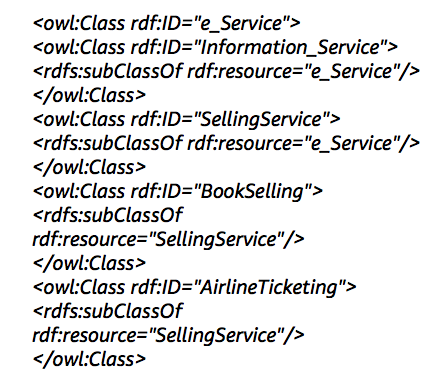
\includegraphics{wscapabilities.png}
\caption{Web services capabilities files (Martin et al. 2007).}
\end{figure}

Figure 1 above shows an extract of web services capabilities taken from Martin et al. (2007). Web services capabilities correspond to functionalities they provide. There are two ways of representing capabilities they explain: the first approach provides an extensive ontology of functions where each class in the ontology corresponds to a class of homogeneous functionalities. In the example above an airline company like British Airways may advertise itself as an airline ticketing selling service, while an online retail business such as Amazon would be a book selling service. The second approach Martin et al. (2007) explain focuses on describing the function from a state transformation perspective. As noted by Peer (2005), this approach is mostly used in artificial intelligence (AI) planning languages such as Planning Definition Domain Language (PDDL). Looking back at our example above Amazon for the second approach may advertise a service that requests a book title, author, address and a valid card payment details, and the state transition occurs as the buyer’s credit card is charged, the book is delivered to her address and changes ownership. Martin et al. (2007) note similarities between the two ways which they claim both use ontologies for representing capabilities in order to provide the link between what the web service does and the general description of the environment in which it operates. Roman et al. (2005) discuss the capability matching process whereby capabilities provided by the advertised web services are compared to the ones that a requesting service is looking for. The goal being to find the advertiser that produces the results required for the requester. In general, it is unrealistic to expect to find an exact match to the query remark Martin et al. (2007). To put things into perspective, they use the example of request for a stock quote service and explain that the matching engine would need to decide whether the needed capability could be fulfilled by say a financial news service. The matchmaker should determine how likely it is that each capability advertisement indicates that the service will accomplish the particular function specified in the query.

\section{The relation between web services discovery and UDDI}

Martin et al. (2007) describe the Universal Discovery and Integration (UDDI) as an initiative that aims to create an internet wide network of registries of web services. UDDI provides a mechanism for providers to advertise their services in terms of API (e.g. endpoint, port) as well as physical contact for providing support about the advertised service. Zhang et al. (2005) define UUDI registry as a language used to specify services features which help in the process of locating, discovering and invoking the service. Martin et al. (2007) stress that UDDI is considered the de facto standard repository of web services in the industry given the backing it has received from renowned hardware and software companies. Mahmood (2007) discusses the weaknesses of UDDI discovery mechanism argue that it does not allow discovering web services based on the functionalities they provide. Another limitation with UDDI is noted by Martin et al. (2007) UDDI is its inability to provide a capability representation language such as the OWL-S Service Profile. As result UDDI supports the location of information about the Web service, once it is known which Web service to use, but it is impossible to locate a Web service only on the basis of what problems it solves argue Martin et al. (2007) who also believe that OWL-S and UDDI complement each other. UDDI provides a worldwide distributed registry that is virtually an industry standard while OWL-S provides the information required for capability matching. The OWL-S/UDDI matchmaker integrates OWL-S capability matching in the UDDI registry. 

\section{Web Services Composition Frameworks}

Rao and Su (2005) in their research work discuss the different web services composition frameworks explaining the different techniques used for composing web services.

\begin{itemize} 
\item \textbf{General framework for web services composition}
This framework is a generic which means that it is not bound to a particular language, platform or algorithm that are used in the composition process. 

\begin{figure}[h!]
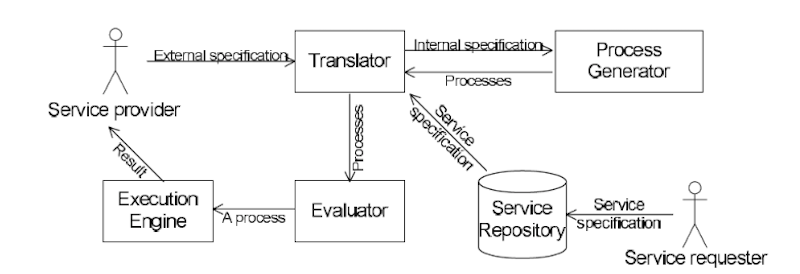
\includegraphics{generic_ws_composition.png}
\caption{Generic web services composition framework (Rao and Su, 2005).}
\end{figure}

The composition system has two kinds of participants as shown in figure 2 above, service provider and service requester. The service providers propose Web services for use while the service requesters consume information or services that are offered by service providers explain Rao and X. Su (2005). The system equally contains the following components: translator, process generator, evaluator, execution engine and service repository. The role of the translator is to provide translation between the internal languages used by the process generator and the external languages used by the participants. For each request, the process generator tries to generate a plan that composes the available services in the service repository to fulfill the request. If more than one plan is found, the evaluator evaluates all plans and proposes the best one for execution. The execution engine executes the plan and returns the result to the service provider. According to Rao and X. Su (2005), the process of automatic service composition includes the following phases:

\textbf{Presentation of Single Service}: the service providers start by advertising their services at a common place like a global marketplace. Languages such as UDDI or DAML-S can be used for advertising. Web service are described by a number of attributes including the signature, states and the non-functional values. Lemos et al. (2016) explain that the signature is represented by the service’s inputs, outputs and exceptions. The signature holds information about any transformation of data during the Web service execution. The states are specified by pre and post-condition and they are modeled as the transformation from one set of states to another in the world (Rao and Su, 2005). Non-functional attributes such as such as cost, service quality and security issues values are used for evaluating the services.

\textbf{Translation of the Languages}: for this phase Rao \& Su (2005) talk about internal and external service specification languages with the former being used by the composition process generator, while the latter is used by service users to express in a simple manner what they can offer or what they want. External service specification languages such as UDDI or DAML-S already exist in the contrary to internal languages where Rao and Su (2005) see the opportunity to develop translation components between the standard Web service languages and the internal languages.

\textbf{Generation of Composition Process Model}: The key component is this phase is the process generator which is responsible for composing the atomic services advertised by the service providers upon receiving a request. The process generator produces a process model as an output which describes the composite service (Rao and Su, 2005). 

\textbf{Evaluation of Composite Service}: This phase is about selecting the composite service that best fit the requirements in cases where more than one composite service is generated for the same requirement. Rao \& Su (2005) discuss the evaluation process which is done based on the overall utilities of each composite service, the most commonly used are utility functions. The best composite service is the one that carries more weight based on the weighting specification provided by the requester for the non-functional attributes.

\textbf{Execution of Composite Service}: This phase is about the execution of the composite service which happens after the evaluation process which leads to one composite process getting selected. Rao and Su (2005) describe this phase “as a sequence of message passing according to the process model”.

\item \textbf{Workflow-based composition}

A method discussed by Ganesarajah \& Lupu (2002) in their paper and further developed by Rao \& Su (2005) who explain that this approach can be done in one of two ways: static or dynamic workflow generation. The key difference between static and dynamic approach is that in the static workflow the requester builds an abstract model before the composition starts whereas for a dynamic composition the creation of the process model and the selection of atomic services are done automatically. An example of static composition is EFlow which uses a graph to model the composite service. Polymorphic Process Model (PPM) is another example discussed by Rao \& Su (2005) that uses a combination of static and dynamic composition. The static setting of PPM is supported by reference process-based multi-enterprise processes, while its dynamic part is supported by service-based processes. The dynamic service composition is enabled by the reasoning based on state machine. Other web service composition techniques using Artificial Intelligence are discussed in the next section.

\item \textbf{Web Service Composition Using AI Planning}

Rao and Su (2005) acknowledge that many research efforts tackling Web service composition problem via AI planning have been reported. They describe planning in general as a five-tuple problem (S, S0, G, A, \textGamma). In the context of web services, S is the set of all possible states of the world, S0 and G are the initial states and the goal states specified in the requirement of Web service requesters. A is a set of available services. \textGamma \space additionally denotes the phase change operate of every service. DAML-S (also called OWL-S in the most recent versions) is the only Web service language that announces the directly connection with AI planning. Rao and Su (2005) explain that the phase change made by the execution of the service is nominal through the precondition and impact properties of the ServiceProfile in DAML-S. Precondition presents logical conditions that ought to be glad before the service being requested. Effects area unit the results of the fortunate execution of a service. Since DAML+OIL, the language accustomed build DAML-S, uses Description Logics as its logical foundation, DAML+OIL has the specific power leaving logical expressions. The majority of the methods reported in this survey use DAML-S as the external Web service description language. There are also a couple of methods that use WSDL or their own languages. Some examples of on a list of Web service composition methods based on AI planning as described by J. Rao and Su X. (2005) which they further classified into five categories including the situation calculus, the Planning Domain Definition Language (PDDL), rule-based planning, the theorem proving and others. \textbf{Situation calculus}: Complex actions are compositions of individual actions. The agent knowledge domain provides a logical encoding of the preconditions and effects of the web service actions within the language of the situation calculus. The agents use procedural programing language constructs composed with ideas outlined for the services and constraints using deductive machinery. 

\textbf{Planning Domain Definition Language (PDDL)}: PDDL is widely recognized as the de facto technique for service composition when planning is needed. Rao and Su (2005) note some similarity and compatibility between DAML-S and PDDL as DAML-S descriptions can be translated into PDDL. This AI planning method offer the possibility for the inputs and outputs parameters to be reusable for the execution of multiple services. A strong interest to Web service composition from AI planning community could be explained roughly by similarity between DAML-S and PDDL representations. PDDL is widely recognized as a standardized input for state-of-the-art planners. Moreover, since DAML-S has been strongly influenced by PDDL language, mapping from one representation to another is straightforward (as long as only declarative information is considered). When planning for service composition is needed, DAML-S descriptions could be translated to PDDL format. AI planning uses closed world assumption which means that if a literal does not exist in the current world, its value is considered to be false. This makes it difficult to express that new information has been acquired during the web service composition process. 

\textbf{Rule-Based Planning}: in this method, more emphasis is placed on the composability rules which consider the syntactic (rules for operations modes and binding protocols for interacting services) and semantic properties of the web services. Semantic rules include the message composability which indicates whether two web services can be composed that is if the output of one is compatible with the input of the other. Then there is the operation semantic composability defining the compatibility between the domains, categories and purposes of the two atomic services. The third subset is the qualitative composability which defines the requesters preferences on the quality of operations for the composite service. The fourth subset is known as composition soundness which specifies whether or not a composition of services is reasonable. The most important thing in this method as noted by Rao and Su (2005) is the composability rules which define the web services attributes that could be used in service composition. One implementation of rule-based planning is SWORD, a developer toolkit for building composite web services using rule-based method. SWORD uses entity relation model instead of standards like WDSL and DMAL-S to specify web services, and it does it by leveraging a service preconditions and postconditions. Rao and Su (2005) stress however that SWORD could lead to uncertain results if the preconditions are functionally dependent on postconditions.

\item \textbf{Web service composition based on code annotation and semantic web services}

Rajasekaran et al. (2005) in their paper present METEOR-S which uses an approach to web service composition based on source code annotation and semantic Web service description. They also discuss WSDL-S, an extension to WSDL 2.0 which is a language specifically designed to incorporate semantic descriptions in WSDL. They note some challenges around standard and inter-operability though they acknowledge that companies have used e-business process definition standards such as RosettaNet and ebXML to provide standardized representation of service functionalities and message exchange formats. While RosettaNet and ebXML provide concrete e-business transaction format, Rajasekaran et al. (2005) recognize their limitation when it comes to logical reasoning inherent in ontological representations. To overcome the limitation METEOR-S employs the use of ontologies based on standards like RosettaNet.

\textbf{METEOR-S}: Rajasekaran et al. (2005) The METEOR is basically a project done at the LSDIS Lab, University of Georgia, focused on workflow management techniques for transactional workflows. It follows on project, which incorporates workflow management for semantic Web services is called METEOR-S. This project uses semantics as key feature for the complete lifecycle of semantic web processes, which represent complex interactions between Semantic Web Services. There are five main stages main stages for creating semantic Web processes including development, annotation, discovery, composition and orchestration. From an architectural point of view, we divide METEOR-S in two main parts – the front end and the back end. The front end, which is the focus of this paper, covers the development, annotation and discovery stages. METEOR-S frontend has 4 main components main components which are the Semantic Web Service Designer, the Semantic Description Generator, the Publishing Interface and the Discovery Engine. 

\pagebreak 

\textbf{The Semantic Web Service Designer}: is graphical user interface (GUI) of METEOR-S which can be used to design and develop Semantic Web Services. It helps design the interface of services and incorporate semantic description 

\begin{figure}[h!]
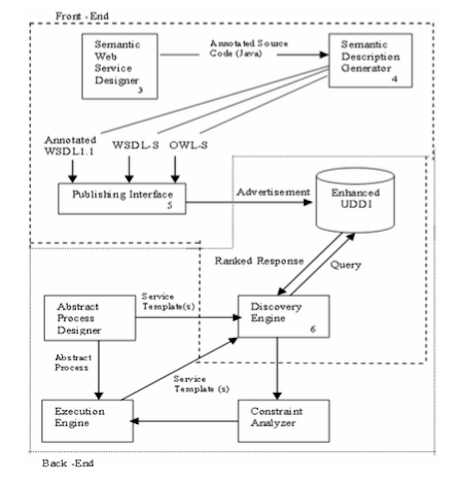
\includegraphics{meteors_arch_diagram.png}
\caption{METEOR-S Architecture diagram (Rajasekaran et al., 2005).}
\end{figure}

\pagebreak 

\textbf{Source Code Annotation} - The output of the ‘Semantic Web Service Designer’ is the annotated source code. Rajasekaran et al. (2005) discuss the example of Oracle and C\#.NET both of which offer features for adding annotations to source code via Javadoc comments and inbuilt metatags, respectively. 

\begin{figure}[h!]
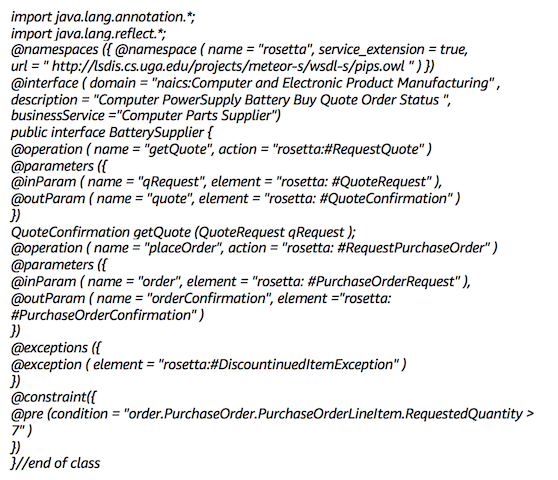
\includegraphics{annotatedjava1.png}
\caption{Sample of annotated Java Source (Rajasekaran et al., 2005).}
\end{figure}

\textbf{Semantic Description Generator} – As a general rule any service requestor can invoke a web service based on its description in the WSDL file. Rajasekaran et al. (2005) however found the description insufficient for user in METEOR-S. They propose extensions to web services description via annotated WSDL 1.1 and WSDL-S files. According to Rajasekaran et al. (2005), the semantic extensions are thought to enhance the discovery and composition of web services. 

\textbf{Discovery Engine} - In METEOR-S makes use of the semantic descriptions and constraints advertised by the service provider to do the discovery (Rajasekaran et al., 2005). The framework uses a template that build the query specifying the functional aspects of the queried service. The template contains information such as operation name, operation action, input and output name and (semantic) type, exception, pre and post conditions, domain, location. The query is used to discover the matching services and is processed by the discovery engine. 
\\
\\
\item \textbf{Medley - An event-driven lightweight platform for service composition} 

Hadj Yahia et al (2016) developed a framework known as Medley which is an event-driven lightweight platform for service composition based on a domain-specific language for describing orchestration and a compiler that produces efficient code. 

To compose services a user would need to specify via Medley Domain Specific Language (DSL) the composition logic and how to assemble the services together. Hadj Yahia et al (2016) explain the mapping that takes place between services and processes in Medley. They further stress that the process workflow is expressed in terms of patterns of events. A user effectively express which process to invoke based on a given event. The written specification is subsequently passed to Medley compiler as input.  The compiler in turn generates the right low-level code which enable communications amongst the assembled processes. Figure 5 below is a code snippet of Medley DSL taken from Hadj Yahia et al (2016) paper.

\begin{figure}[ht]
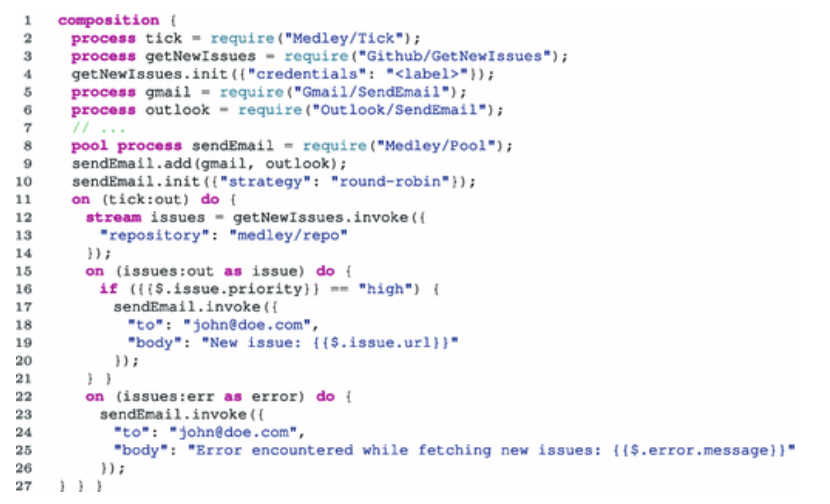
\includegraphics{medley.png}
\caption{A composition example using MEDLEY DSL (Hadj Yahia, 2016).}
\end{figure}

\end{itemize}

\pagebreak 

\section{References}
\begin{enumerate}
\item Barros, Alistair, et al. “Standards for Web Service Choreography and Orchestration: Status and Perspectives.” Business Process Management Workshops Lecture Notes in Computer Science, 2006, pp. 61–74.

\item Baryannis G. et al. (2010) Service Composition. In: Papazoglou M.P., Pohl K., Parkin M., Metzger A. (eds) Service Research Challenges and Solutions for the Future Internet. Lecture Notes in Computer Science, vol 6500. Springer, Berlin, Heidelberg

\item Ben Hadj Yahia, Elyas \& Reveillere, L \& Yerom, Bromberg \& Chevalier, Raphaël \& Cadot, Alain. (2016). Medley: An Event-Driven Lightweight Platform for Service Composition. LNCS. 9671. 3-20.

\item Biswas D. (2005) Compensation in the World of Web Services Composition. In: Cardoso J., Sheth A. (eds) Semantic Web Services and Web Process Composition. SWSWPC 2004. Lecture Notes in Computer Science, vol 3387. Springer, Berlin, Heidelberg

\item Cardoso J., Miller J., Su J., Pollock J. (2005) Academic and Industrial Research: Do Their Approaches Differ in Adding Semantics to Web Services?. In: Cardoso J., Sheth A. (eds) Semantic Web Services and Web Process Composition. SWSWPC 2004. Lecture Notes in Computer Science, vol 3387. Springer, Berlin, Heidelberg

\item D Jordan, J Evdemon, A Alves, A Arkin. Web services business process execution language version 2.0, https://docs.oasis-open.org/wsbpel/2.0/PR02/wsbpel-specification-draft-diff.pdf  retrieved on 15th March 2019

\item D Roman, U Keller, H Lausen, J De Bruijn, Web service modeling ontology
2005 - content.iospress.com

\item Dustdar, Schahram, and Wolfgang Schreiner. “A Survey on Web Services Composition.” International Journal of Web and Grid Services, vol. 1, no. 1, 2005, p. 1.

\item Ganesarajah, D., \& Lupu, E. (2002). Workflow-based composition of Web-services: a business model or a programming paradigm? Proceedings. Sixth International Enterprise Distributed Object Computing.

\item H Kreger, 2001. “Web services conceptual architecture (WSCA 1.0).”  IBM software group,researchgate.net

\item Klusch, Matthine. “Semantic Web Service Coordination.” CASCOM: Intelligent Service Coordination in the Semantic Web, pp. 59–104.

\item LA Digiampietri, JJ Pérez-Alcázar, CB Medeiros, 2007. AI Planning in Web Services Composition: a review of current approaches and a new solution, researchgate.net

\item Liu, Jiamao, et al. “Service Registration and Discovery in a Domain-Oriented UDDI Registry.” The Fifth International Conference on Computer and Information Technology (CIT05), 2005

\item Lemos, A. L., Daniel, F. \& Benatallah, B. Web Service Composition: A Survey of Techniques and Tools. ACM Comput. Surv. 48, 33:1-33:41 (2015).

\item Louridas, Panagiotis. “Orchestrating Web Services with BPEL.” IEEE Software, vol. 25, no. 2, 2008, pp. 85–87.

\item Mabrouk, Nebil Ben, et al. “QoS-Aware Service Composition in Dynamic Service Oriented Environments.” Middleware 2009 Lecture Notes in Computer Science, 2009, pp. 123–142.

\item Martin, D., Burstein, M., McDermott, D. et al. World Wide Web (2007) 10: 243. \url{https://doi.org/10.1007/s11280-007-0033-x} 

\item Nakajima, Shin. “Model-Checking Behavioral Specification of BPEL Applications.” Electronic Notes in Theoretical Computer Science, vol. 151, no. 2, 2006, pp. 89–105.

\item Pahl, Claus, and Yaoling Zhu. “A Semantical Framework for the Orchestration and Choreography of Web Services.” Electronic Notes in Theoretical Computer Science, vol. 151, no. 2, 2006, pp. 3–18.

\item Peer, Joachim. “A PDDL Based Tool for Automatic Web Service Composition.” Principles and Practice of Semantic Web Reasoning Lecture Notes in Computer Science, 2004, pp. 149–163.

\item Rajasekaran P., Miller J., Verma K., Sheth A. (2005) Enhancing Web Services Description and Discovery to Facilitate Composition. In: Cardoso J., Sheth A. (eds) Semantic Web Services and Web Process Composition. SWSWPC 2004. Lecture Notes in Computer Science, vol 3387. Springer, Berlin, Heidelberg

\item Rao J., Su X. (2005) A Survey of Automated Web Service Composition Methods. In: Cardoso J., Sheth A. (eds) Semantic Web Services and Web Process Composition. SWSWPC 2004. Lecture Notes in Computer Science, vol 3387. Springer, Berlin, Heidelberg

\item Schmidt, C. \& Parashar, M. World Wide Web (2004) 7: 211. \url{https://doi.org/10.1023/B:WWWJ.0000017210.55153.3d} retrieved on 18th April 2019

\item Strunk, Anja. “QoS-Aware Service Composition: A Survey.” 2010 Eighth IEEE European Conference on Web Services, 2010.

\item The promise and limitations of service-oriented architecture
Z Mahmood - International journal of Computers, 2007 - INTERNATIONAL JOURNAL OF COMPUTERS, Issue 3, Volume 1, 2007.

\end{enumerate}
\end{document}

